\section{Evaluation}

\subsection{Experiment Setup}


\subsection{Results}

\begin{figure}
\centering
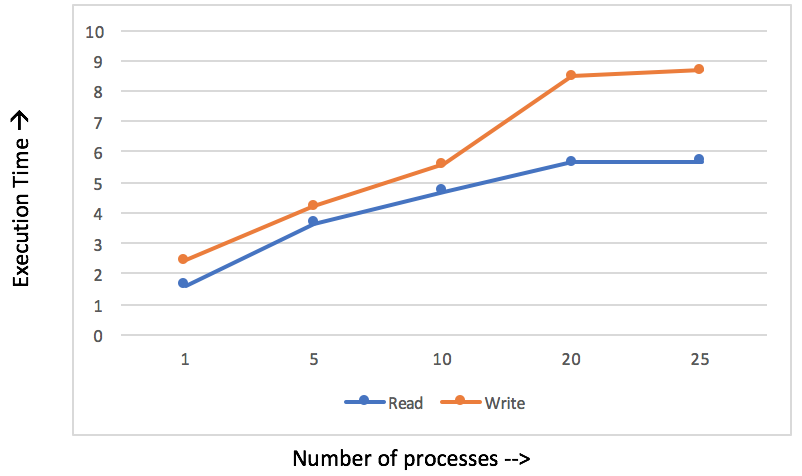
\includegraphics[height=2in, width=3.2in]{images/OneClient.png}
\caption{Execution time (in ms) of 1000 READ and WRITE requests generated from each process running in a single client. These requests perform action on the same file.}
\end{figure}

\begin{figure}
\centering
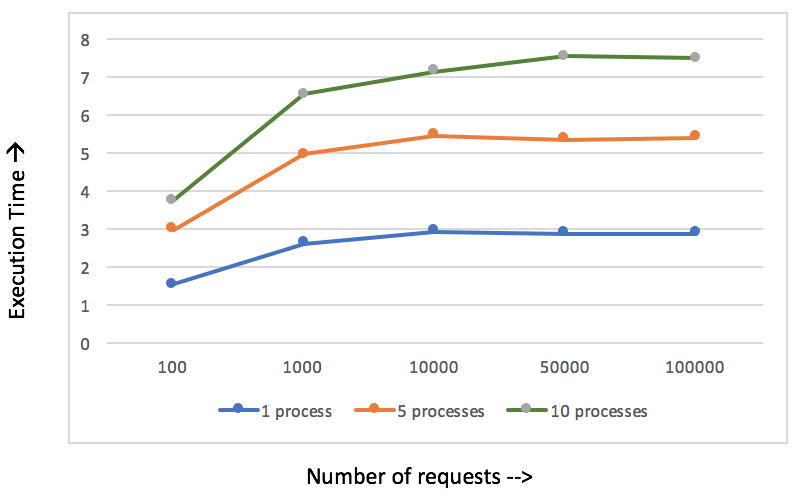
\includegraphics[height=2in, width=3.2in]{images/FiveClient_Read.png}
\caption{Execution time (in ms) of increasing number of READ requests generated from each process running in 5 clients. These requests perform action on the same file.}
\end{figure}

\begin{figure}
\centering
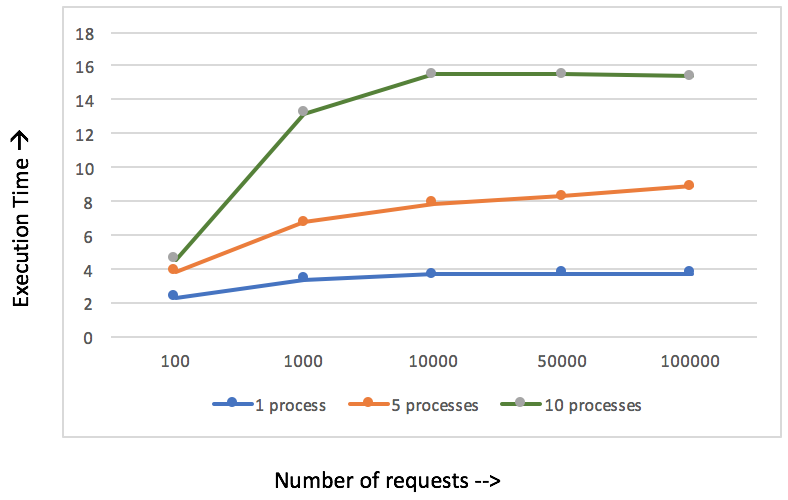
\includegraphics[height=2in, width=3.2in]{images/FiveClient_Write.png}
\caption{Execution time (in ms) of increasing number of WRITE requests generated from each process running in 5 clients. These requests perform action on the same file.}
\end{figure}

\begin{figure}
\centering
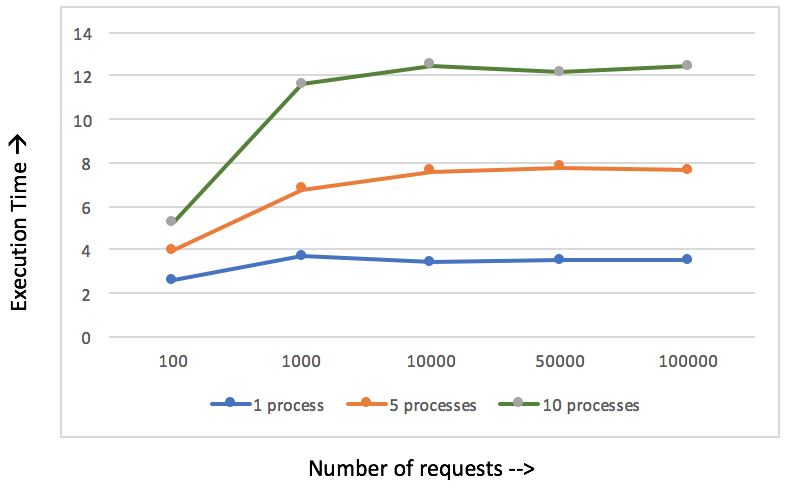
\includegraphics[height=2in, width=3.2in]{images/FiveClient_RW.png}
\caption{Execution time (in ms) of equal and increasing number of READ and WRITE requests generated from each process running in 5 clients. These requests perform action on the same file.}
\end{figure}

\begin{figure}
\centering
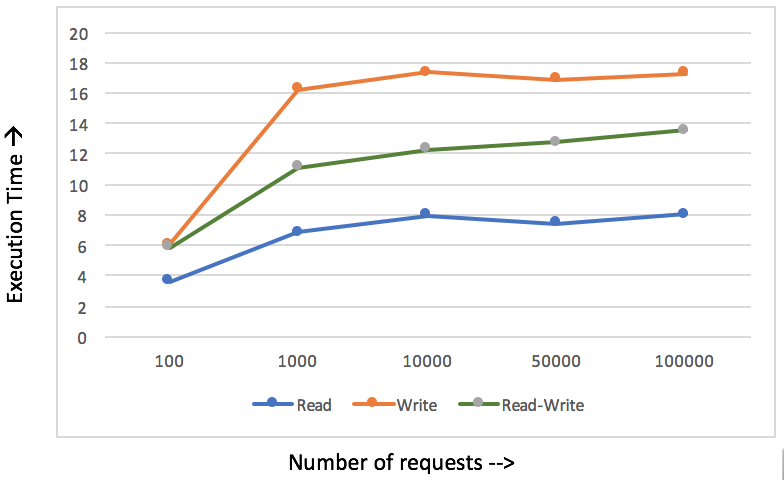
\includegraphics[height=2in, width=3.2in]{images/FiveClient_DiffFile.png}
\caption{Execution time (in ms) of increasing number of READ and WRITE requests generated from each process running in 5 clients. These requests perform action on different files.}
\end{figure}








